% To convert to svg
% lualatex --output-format=dvi filename.tex
% dvisvgm filename.dvi
%\documentclass[a3paper]{article}
%\usepackage[left=0mm,top=1cm,right=0mm,bottom=0mm]{geometry}
\documentclass[border=0]{standalone}
% \documentclass[dvisvgm]{minimal}
\usepackage{tikz}
\usetikzlibrary{calc}
\usepackage{xkcdcolors}
% \definecolor{pGreen}{HTML}{006633}
% \definecolor{pRed}{HTML}{cc0033}
\usepackage{pgfplots}
\pgfplotsset{compat=1.18}
\tikzset{
        speaker/.pic={
        \draw (-1,-1) --++ (0.5,0) --++ (1.5,-1)--++(0,3)--++(-1.5,-1)--++(-0.5,0);
        \node[text width=2cm] at (0,-.5) {Source of sound}; 
    }
}
\begin{document}
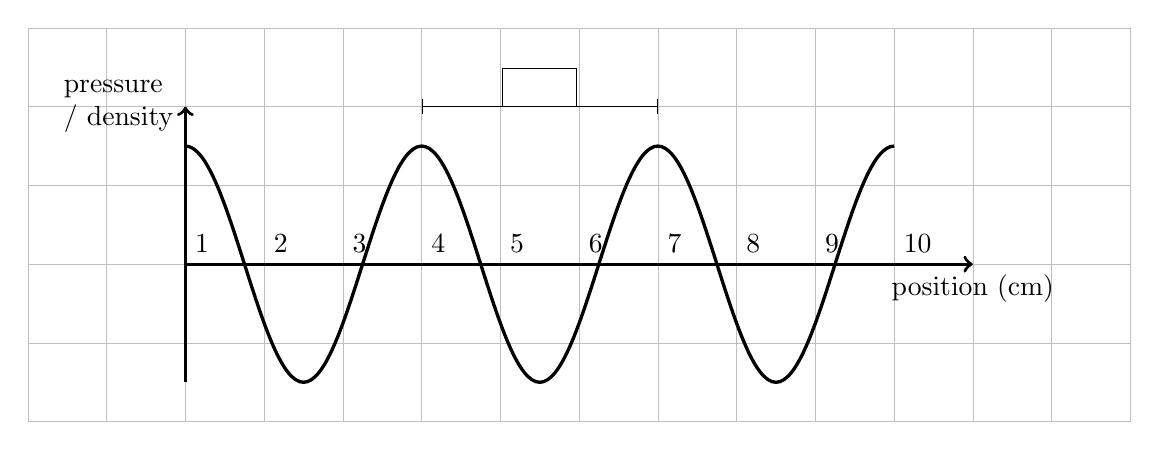
\begin{tikzpicture}
    \draw[yshift=0.5cm,very thin,gray!50] (-1,-3) grid (13,2);
        \pgfmathsetmacro{\w}{3}
        \pgfmathsetmacro{\d}{0}
        \foreach \i in {1,2,3,...,10}{
          \node[below right] at (\i,0) {\i};
        %   \node[below] at ({1+(\i-1)*\w+\w/2},-2) {R};
          }
        %   \node[below] at ({1+3*\w},-2) {C};
          \draw[very thick] (1,{1+\d}) cos (1.75,{-.5+\d}) sin (2.5,{-2+\d}) cos (3.25,{-.5+\d}) sin (4,{1+\d}) cos (4.75,{-.5+\d}) sin (5.5,{-2+\d}) cos (6.25,{-.5+\d}) sin (7,{1+\d}) cos (7.75,{-.5+\d}) sin (8.5,{-2+\d}) cos (9.25,{-.5+\d}) sin (10,{1+\d});
          \draw[very thick,->] (1,{-.5+\d}) -- (11,{-.5+\d}) node[below] {position (cm)};
          \draw[very thick,->] (1,{-2+\d}) -- (1,{1.5+\d}) node[left,text width=4em] {pressure / density};
          \draw[|-|,yshift=1.5cm] (4,0) -- ++(3,0) node[midway,above,text=white,fill=white,draw,text width=2em] {$\lambda$};

    \end{tikzpicture}
\end{document}
